% Author: Animesh Garg
% Date: July 15, 2013

\section{PROBLEM STATEMENT}
\label{sec:problemStatement}

The problem of minimizing discomfort in medical fixtures can be modeled as a 
form closure grasping problem with bounded contact wrench at any contact point.

We are given input a surface mesh, $M$ of the body volume, $V$ required to be 
fixed. The mesh $M$ can be generated using MRI/CT scanning. Gravity vector ($g$) is also provided as input. The required output
 of the algorithm is the subset of points, $S_{opt}$ on the surface mesh which 
 are required for form closure with bounded contact wrench, $w_{ub}$. 

Thereafter, only using points in $S_{opt}$ we construct a fixture, $F$ to hold the 
body volume $V$. The fixture, $F$ is then physically created using 3D-printing. 
The fixture $F$ may consist of multiple pieces, which need assembly over body 
volume $V$. The fixture assembly on the body volume $V$ is in principle 
guaranteed to hold $V$ in form closure. 

\begin{figure}[t!]
  \begin{center}
    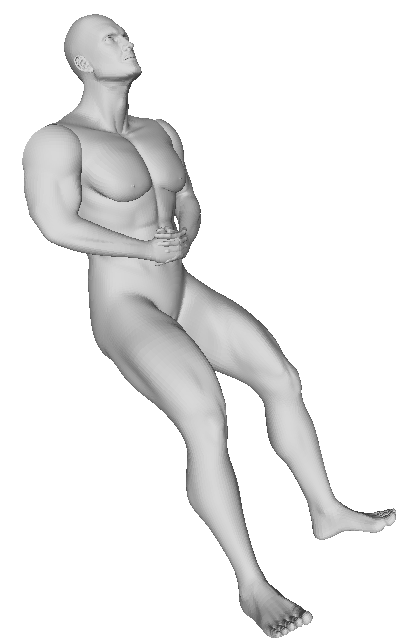
\includegraphics[width=0.6\linewidth]{images/maleBody}
  \end{center}
  \vspace{-10pt}
\caption{ The figure shows a commercially available high fidelity mesh of a human male body. We will use this model for evaluation of proposed algorithmic fixturing techniques in this paper.}
  \vspace*{-15pt}
  \label{fig:maleBody}
\end{figure}


We will evaluate the results using a standard commercially available human body 
mesh for experimentation as shown in figure~\ref{fig:maleBody}\todo{ask Sachin about origins of the model.} Quality 
of algorithmically generated fixtures will be measured for head and limb 
fixturing in virtual environments for varying number of contacts and varying the upper bound on contact wrench, $w_{ub}$.

Furthermore, we will 3D print the head and a portion of torso to mimic the patient in supine position. We will also create a custom head fixture for physical assessment of the proposed fixtures. 